\section{Reflected Cross Site Scripting (XSS)}
\paragraph{Vulnerabilidad} Cross-Site Scripting es un tipo de inyección en el cual un
script malicioso es inyectado en la web. En este caso nos centramos en el {\it reflected}, 
el cual consiste en ejecutar el script desde entradas de la web sin validar. En nuestro caso 
trataremos de obtener las cookies de sesión mediante este ataque.
\paragraph{Nivel bajo} En esta pantalla se nos muestra únicamente un input,
por lo que será nuestro único punto de ataque. Lo primero que haremos será comprobar que permite ejecutar
scripts introduciendo la siguiente entrada: 
\begin{lstlisting}
    <script>alert("hola")</script>
\end{lstlisting}
En él únicamente tratamos de lanzar un {\it pop-up} con el texto hola.
En la figura \ref{fig:hola} vemos el resultado obtenido de introducir dicha entrada, el cual
 ha sido satisfactorio.
\begin{figure}[ht!]
    \centering
    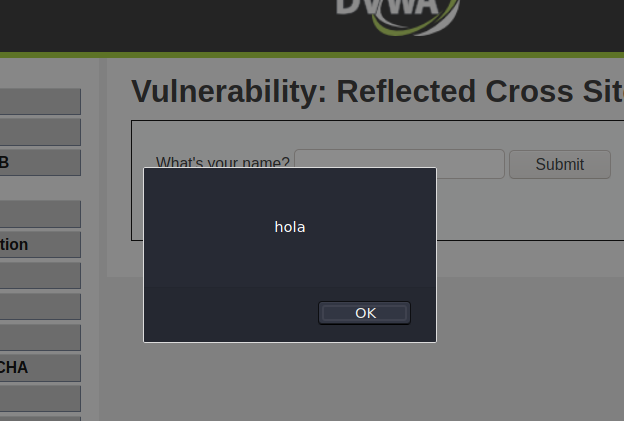
\includegraphics[width=14cm]{img/xss/hola.png}
    \caption{Pop-up Hola}
    \label{fig:hola}
\end{figure}

Para obtener las claves de sesión modificamos un poco la entrada para mostrar en el {\it pop-up}
los datos deseados en vez de un texto arbitrario, quedando la nueva entrada de la siguiente forma:
\begin{lstlisting}
    <script>alert(document.cookie)</script>
\end{lstlisting}
Con ello logramos obtener las claves como se muestra en la figura \ref{fig:low}. 
\begin{figure}[ht!]
    \centering
    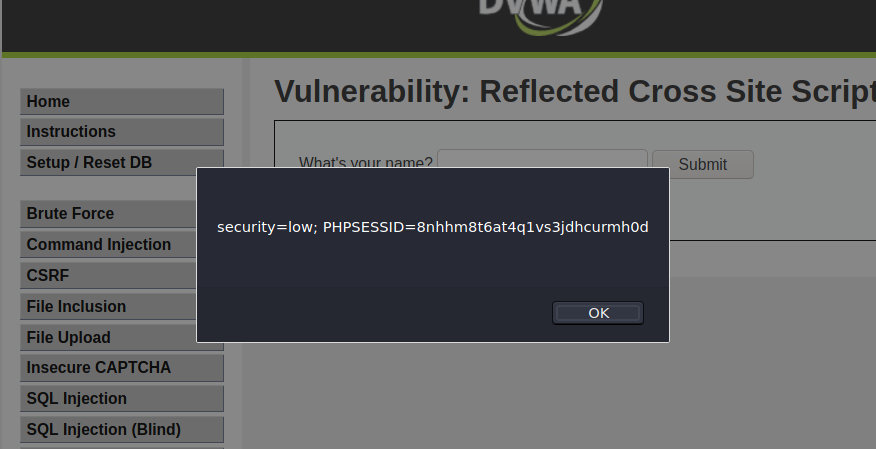
\includegraphics[width=14cm]{img/xss/low.png}
    \caption{Obtención de claves a nivel bajo}
    \label{fig:low}
\end{figure}
Este ataque ha tenido existo dado que no se aplica ningún filtro  en la entrada,
posiblemente en niveles superiores no servirá este ataque dado que habrá una expresión regular
que valide la entrada

\paragraph{Nivel medio} La idea de este nivel es evitar una posible validación por expresión regular. 
La más simple sería una que permita todas las entradas menos las que contengan la palabra {\it script}, por
lo que tratamos de modificar la entrada de la siguiente forma:
\begin{lstlisting}
    <sCriPt>alert(document.cookie)</ScripT>
\end{lstlisting}
El resultado fue satisfactorio, dado que únicamente controlan que no esté la palabra {\it script}, pero 
al modificarlo y no ser {\it Case sensitive} el {\it html} se obtuvo las credenciales. No se ha considerado necesario 
poner una captura del resultado dado que el resultado es el mismo que en la figura \ref{fig:low} pero con otro
ID de sesión. Este ataque no funcionará en niveles superiores porque tendrán una mejor expresión regular
que evitará cualquier forma de la palabra script.

\paragraph{Nivel alto} Para este nivel tuvimos que buscar la manera de obtener un {\it alert dialog} sin usar la 
palabra {\it script}. Para ello nos ayudamos de una {\it cheat sheet} en Github \cite{xsscheatsheet}. En ella vimos
que una forma de obtener un {\it alert dialog} es provocar un error al mostrar una imagen y al ejecutarse la función
de {\it callback} por el error mostrarlo, de esta forma creamos la siguiente entrada:
\begin{lstlisting}
    <img src="image.gif" onerror=alert(document.cookie)>
\end{lstlisting}
Con esta entrada logramos las credenciales. En niveles superiores no funcionará porque 
posiblemente eliminen los caracteres especiales, dejando únicamente que se introduzcan alfanuméricos, de tal forma 
que sea imposible usar elementos de {\it html}, ya que empiezan y acaban por símbolos especiales.
